\section{Budowa aplikacji}
\begin{figure}[H]
	\centering
	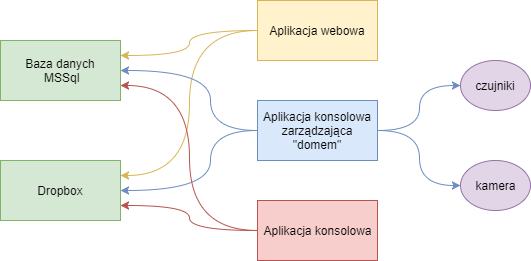
\includegraphics[scale=0.8]{schemat_systemu.png}
	\caption{Budowa systemu zarządzania domem}
	\label{fig:schemat_systemu}
\end{figure}
Aplikację powstałą na potrzeby tej pracy można podzielić na 3 moduły, które zostały przedstawione na rysunku \ref{fig:schemat_systemu}, a składają się na nie :
\begin{itemize}
\item Aplikacja webowa- interfejs pozwalający na zlecanie nowych zadań aplikacji konsolowej oraz odczyt wyników przesłanych przez nią oraz przez program zarządzający domem,
\item Aplikacja konsolowa- przetwarza zadania detekcji oraz rozpoznawania twarzy zlecone za pomocą aplikacji webowej,
\item Program zarządzający domem- przekazuje cyklicznie odczytywane dane z czujników oraz wykryte ruchy do bazy danych, w celu dalszej obróbki przez pozostałe moduły.
\end{itemize}
Na usługi pomocnicze wykorzystane w projekcie składają się
\begin{itemize}
\item baza danych- przechowywanie danych o dodanych zadaniach, wynikach, nauczonych sieciach neuronowych oraz osobach,
\item dropbox- przechowywanie większych plików- obrazów oraz nauczonych modeli sieci.
\end{itemize}

\subsection{Wzorzec projektowy MVC}
\begin{figure}[H]
	\centering
	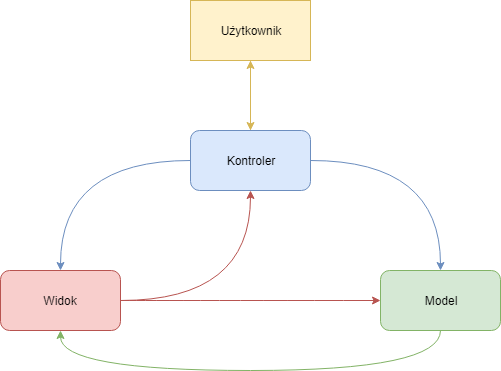
\includegraphics[scale=0.8]{mvc.png}
	\caption{Schemat klasycznego wzorca MVC}
	\label{fig:schemat_mvc}
\end{figure}
Strona internetowa powstała na bazie bardzo popularnego wśród programistów wzorca projektowego MVC. Założenia wzorca Model-Widok-Kontroler są bardzo proste, ich składowymi są:
\begin{itemize}
\item Model- reprezentuje logikę biznesową. Tutaj znajdują się wszelkie obiekty, które służą do wykonywania zaimplementowanej funkcjonalności danej aplikacji,
\item Widok- jest warstwą prezentacji. Odpowiada za prezentację logiki biznesowej (Modelu) użytkownikowi w przystępny sposób,
\item Kontroler- obsługuje żądania użytkownika. Odebrane zadania oddelegowuje do odpowiednich modeli.
\end{itemize}

\subsection{Single Page Application}
Single Page Application (SPA) to aplikacja lub strona internetowa, która w całości wczytuje się za jednym razem. Cały potrzebny do działania strony kod (HTML, CSS, JavaScript) przesyłany jest na początku lub dodawany dynamicznie w kawałkach, zwykle w odpowiedzi na interakcje generowane przez użytkownika.
Sposób działania takiej aplikacji jest zbliżony do odczuć towarzyszących korzystaniu z aplikacji desktopowej lub mobilnej.

\section{Raspberry Pi}
Raspberry Pi jest platformą komputerową stworzoną przez Raspberry Pi Foundation, na którą składa się pojedynczy obwód drukowany. Pierwsza wersja tego urządzenia została zaprezentowana w 2012 roku. Na potrzeby tej pracy wykorzystano nowszą wersję urządzanie w wersji 3 B, którą została wyposażona w 4 rdzeniowy procesor i 1 GB pamięci RAM. Raspberry pozwala na podłączenie wielu urządzeń peryferyjnych za pomocą 4 portów USB lub 40 pinów GPIO. Dodatkowe złącze pozwala na podłączenie dedykowanej kamery. Dzięki znacznej ilości portów GPIO istnieje możliwość komunikacji cyfrowej z sensorami. Budowa urządzenia nie pozwala na podłączenie czujników analogowych.
\begin{figure}[H]
	\centering
	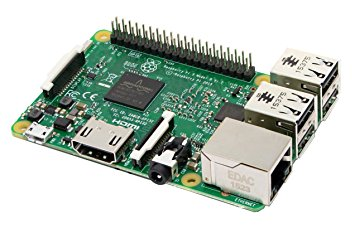
\includegraphics[scale=0.7]{raspberrypi.jpg}
	\caption{Raspberry Pi 3 B}
	\label{fig:raspberrypi}
\end{figure}

\section{Open Cv}
OpenCv (Open Source Computer Vision Library) jest open sourcową biblioteką napisaną w języku C. Udostępniono liczne interfejsy biblioteki pozwalające na pracę z nią miedzy innymi w języku C++ i Python. Biblioteka wspiera systemy operacyjne Linux oraz Windows. Biblioteka została ukierunkowana na przetwarzanie obrazu w czasie rzeczywistym. W licznie udostępnionych funkcjach można znaleźć moduły pozwalające na detekcję i rozpoznawanie twarzy na obrazie, które zostały szerzej opisane w kolejnym punkcie.

\subsection{Detekcja twarzy}
Głównym wykrywaczem twarzy wykorzystywanym przez OpenCv jest kaskadowy klasyfikator Haar'a ale poza nim istnieją również inne metody. Jedną z nich jest wykorzystanie głębokiej sieci neuronowej.

\subsubsection{Klasyfikator kaskad Haar'a} \label{haar}
Detekcja obiektów klasyfikatorem kaskad Haar'a została oparta o metodę Paul'a Viola i Michael'a Jones'a– w skrócie Viola-Jones.

\subsubsection{Algorytm Viola-Jones}
Jest to jeden z pierwszych algorytmów pozwalających na osiągnięcie zadowalających wyników w detekcji obiektów na obrazie. Został on zaproponowany w 2001 roku i został przemyślany z głównym przeznaczeniem dla detekcji twarzy. Na kluczowe koncepcje tej metody składają się:
\begin{itemize}
\item wyszukiwanie cech Haar'a,
\item integralność obrazu,
\item metoda uczenia AdaBoost (podstawowy algorytm do boostingu, metoda dzięki której z dużej liczby słabych klasyfikatorów można otrzymać jeden lepszy )
\end{itemize}

\subsubsection{Cechy Haar'a}
Cechy wykorzystywane w metodzie Viola-Jones opierają się na falkach Haara. Falki Haara są to sekwencje przeskalowanych kwadrato-podobnych funkcji, które razem tworzą falę(falo-podobną oscylację), podstawę z której można zbudować kwadrat. W dwóch wymiarach, fala kwadratu jest parą przylegających do siebie prostokątów, gdzie jeden jest jaśniejszy, a drugi ciemniejszy.
\begin{figure}[H]
	\centering
	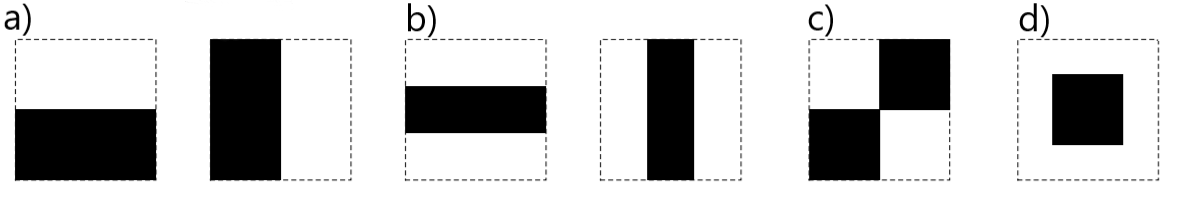
\includegraphics[scale=0.4]{szablon_cech_haara.png}
	\caption{Szablony cech Haar'a}
	\label{fig:szablon_cech_haara}
\end{figure}
Wartość każdej cechy jest obliczana jako różnica sumy poziomów szarości pikseli pokrywanych przez biały oraz czarny prostokąt oraz sumy poziomów szarości pikseli pokrywanych przez czarny prostokąt. Składniki tej różnicy posiadają wagi odwrotnie proporcjonalne do rozmiarów, dzięki czemu różnice wielkości dwóch obszarów są kompensowane.

\subsubsection{Głęboka sieć neuronowa} \label{dnn}
Pojęciem uczenia maszynowego określa się dziedzinę nauk związanych ze sztuczną inteligencją, zajmującą się badaniem algorytmów i systemów, które usprawniają swoje działanie wraz ze zdobywaniem nowej wiedzy lub też doświadczeniem. Wiedzą określamy dane uczące, które zostały wykorzystane do nauki. System może zostać usprawniony poprzez zwiększenie wiedzy systemu, które powinno pozwolić na usprawnienie procesu rozwiązywania podstawowych problemów.

Algorytmy głębokiego uczenia maszynowego są jednymi z najbardziej zaawansowanych. Zbudowane są one w sposób przypominający biologiczne sieci neuronowe. Głęboka sieć neuronowa składa się z neuronów rozmieszczonych na warstwach. Wiele warstw jest powodem dla którego taki rodzaj algorytmu określa się mianem głębokiego. Przykładowa budowa głębokiej sieci neuronowej została przedstawiona na rysunku \ref{fig:budowa_dnn}.
\begin{figure}[H]
	\centering
	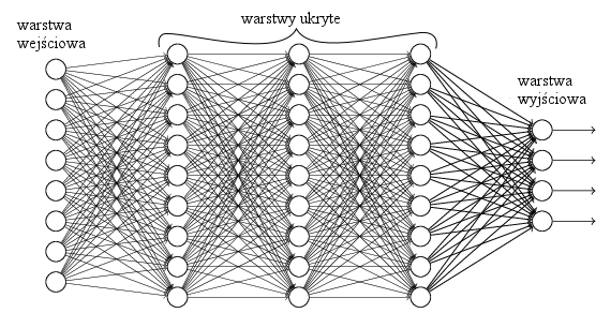
\includegraphics[scale=0.6]{schemat_dnn.png}
	\caption{Budowa głębokiej sieci neuronowej}
	\label{fig:budowa_dnn}
\end{figure}
Każdy z takich “sztucznych neuronów” jest tak naprawdę informacją, która jest przesyłana dalej do następnych neuronów i ich warstw. Poszczególne warstwy “uczą” się przetwarzać kolejne cechy obiektów/obrazów/dźwięków itp., dzięki czemu są w stanie odtwarzać całe obiekty w bardzo rzeczywisty sposób.

\subsection{Rozpoznawanie twarzy}
\subsubsection{Eigen} \label{eigen}
\subsubsection{Fisher} \label{fisher}
\subsubsection{LBPH} \label{lbph}

\section{Azure}
\subsection{Cognitive Services} \label{cognitive_services}

\section{AWS}

